\documentclass[../wassersteinmetrik.tex]{subfiles}

\begin{document}
	
	\begin{figure}[H]
		\centering
		\begin{subfigure}[t]{0.5\textwidth}
			\centering
			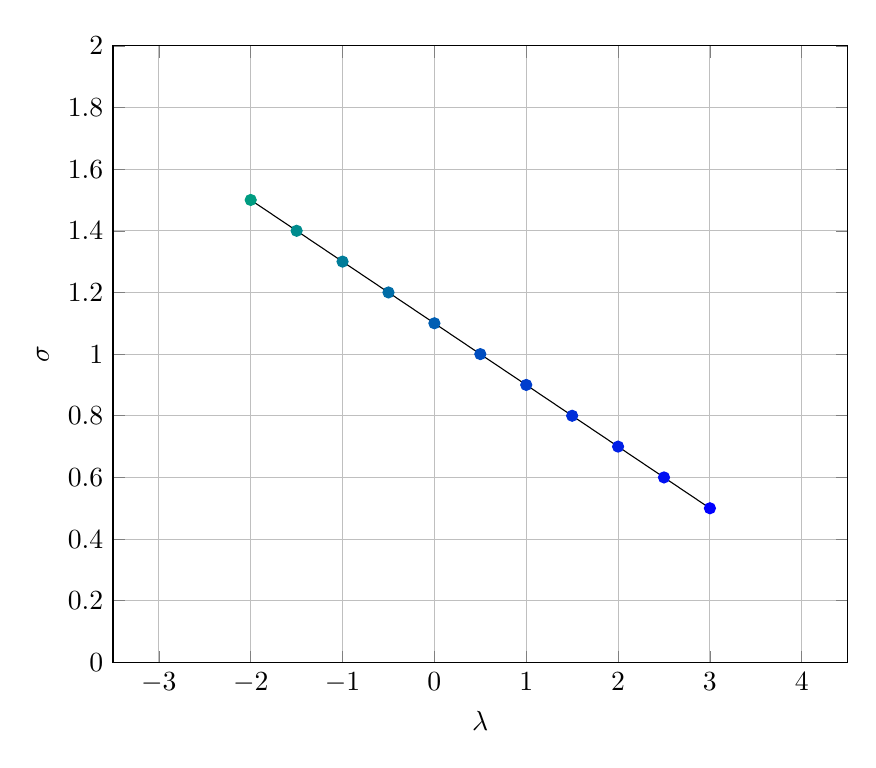
\begin{tikzpicture}[define rgb/.code={\definecolor{mycolor}{RGB}{#1}},
				rgb color/.style={define rgb={#1},mycolor}]
				
				\def\startlambda{-2}
				\def\endlambda{3}
				\def\startsigma{1.5}
				\def\endsigma{0.5}
				\def\steps{10}
				\definecolor{startcolor}{RGB}{0,156,129}
				\definecolor{endcolor}{RGB}{0,0,255}
				
				\begin{axis}[
					grid=major,
					xmax=4.5, ymax=2, xmin=-3.5, ymin=0,
					width=0.9\textwidth,
					xlabel={$\lambda$},
					ylabel={$\sigma$}
					]
					\draw (axis cs:-2, 1.5) -- (axis cs:3, 0.5);
					
					\addplot[rgb color={  0, 156, 129}, mark=*] coordinates {(-2  , 1.5)};
					\addplot[rgb color={  0, 140, 142}, mark=*] coordinates {(-1.5, 1.4)};
					\addplot[rgb color={  0, 125, 154}, mark=*] coordinates {(-1  , 1.3)};
					\addplot[rgb color={  0, 109, 167}, mark=*] coordinates {(-0.5, 1.2)};
					\addplot[rgb color={  0,  94, 179}, mark=*] coordinates {( 0  , 1.1)};
					\addplot[rgb color={  0,  78, 192}, mark=*] coordinates {( 0.5, 1.0)};
					\addplot[rgb color={  0,  62, 205}, mark=*] coordinates {( 1  , 0.9)};
					\addplot[rgb color={  0,  47, 217}, mark=*] coordinates {( 1.5, 0.8)};
					\addplot[rgb color={  0,  31, 230}, mark=*] coordinates {( 2  , 0.7)};
					\addplot[rgb color={  0,  16, 242}, mark=*] coordinates {( 2.5, 0.6)};
					\addplot[rgb color={  0,   0, 255}, mark=*] coordinates {( 3  , 0.5)};
				\end{axis}
			\end{tikzpicture}
			\caption{Parametervektor $(\lambda, \sigma) \in \R \times (0, \infty)$.}
			\label{Fig:SubLeft}
		\end{subfigure}%
		~ 
		\begin{subfigure}[t]{0.5\textwidth}
			\centering
			\begin{tikzpicture}
				
				\def\startlambda{-2}
				\def\endlambda{3}
				\def\startsigma{1.5}
				\def\endsigma{0.5}
				\def\steps{10}
				\definecolor{startcolor}{RGB}{0,156,129}
				\definecolor{endcolor}{RGB}{0,0,255}
				
				\begin{axis}[
					grid=major,
					xmax=5, ymax=1, xmin=-5, ymin=0, samples=200,
					width=0.9\textwidth,
					xlabel={$x$},
					ylabel={$f_{\lambda,\sigma}(x)$}
					]
					\foreach [evaluate=\t as \v using (\t)*100/(\steps)] \t in {0,...,\steps}
					{
						\def\lambda{\startlambda + \t * (\endlambda - \startlambda) / \steps}
						\def\sigma{\startsigma + \t * (\endsigma - \startsigma) / \steps}
						
						\edef\temp{\noexpand
							\addplot[endcolor!\v!startcolor, thick]{gauss(x, \lambda, \sigma)};
							\noexpand}\temp
					}
				\end{axis}
			\end{tikzpicture}
			\caption{Dichten $f_{\lambda,\sigma}$ von $\mathcal{N}(\lambda, \sigma)$.}
			\label{Fig:SubRight}
		\end{subfigure}
		\caption{Visualisierung von $\mathcal{N}$.}
		\label{Fig:Main1}
	\end{figure}
	
\end{document}